\subsubsection{Advising Dataset}

The Advising dataset\cite{finegan-dollak-etal-2018-improving} was created in order to propose improvements in Text-to-SQL systems. The creators of the dataset compare human-generated and automatically generated questions, citing properties of queries that relate to real-world applications. The dataset consists of questions from the University of Michigan students about courses that lead to particularly complex queries. The data is obtained from a fictional student database which includes student profile information such as recommended courses, grades, and previous courses. Moreover, in order to obtain the data for the dataset, academic advising meetings were conducted where students were asked to formulate questions they would ask if they knew the database. After obtaining the questions, the creators of the dataset compared the query results with those from other datasets such as ATIS [\ref{sec:atis}], GeoQuery, and Scholar. Many of the queries in the Advising dataset were the same as those found in the other datasets.

% \begin{figure}[H]
%     \centering
%     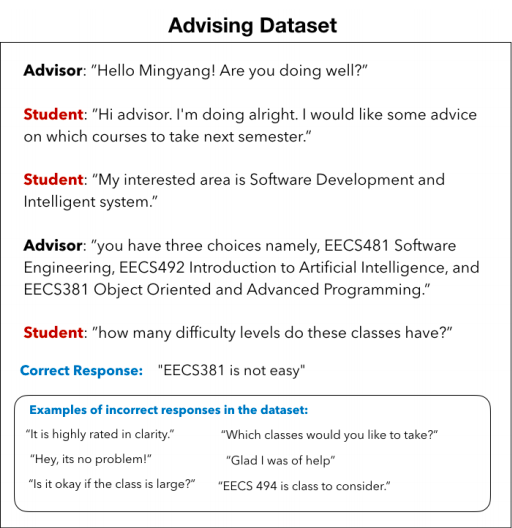
\includegraphics[width=0.5\textwidth]{pics/db/Advising.png}
%     \caption{Example from Advising dataset \cite{vig_comparison_2019}}
%     \label{fig:Advising}
% \end{figure}